\documentclass[a4paper,11pt,titlepage]{article}

\usepackage{ucs}
% per input encoding kann man Umlaute direkt einsetzten, aber  dann ist man von Font des jeweiligen Rechners abh"angig. Daher mag ich es nicht!
%\usepackage[utf8x]{inputenc}
\usepackage[german,ngerman]{babel}
\usepackage{fontenc}
\usepackage[pdftex]{graphicx}
%\usepackage{latexsym}
\usepackage[pdftex]{hyperref}
\usepackage{listings}
\usepackage{xcolor}
\usepackage[landscape]{geometry}

\definecolor{dunkelblau}{RGB}{16, 55, 188}
\definecolor{orange}{RGB}{255, 60, 0}
\definecolor{gruen}{RGB}{18, 118, 34}
\definecolor{gelb}{RGB}{255, 200, 0}
\definecolor{lila}{RGB}{147, 18, 114}

\lstdefinestyle{python}{
language=python,
commentstyle=\color{gruen}, 
keywordstyle =\color{dunkelblau}, 
stringstyle=\color{orange},
literate=
    {\{}{{\textcolor{gelb}{\{}}}1
    {\}}{{\textcolor{gelb}{\}}}}1
    {[}{{\textcolor{lila}{[}}}1
    {]}{{\textcolor{lila}{]}}}1,
%Bis hier hin Farbgebung
breaklines=true, %Zeilenumbruch
frame=single, % Umrandung des Codes
rulecolor=\color{lightgray},
numbers=left, % Nummerierung hinzufügen (links)
numberstyle=\tiny, % Stil der Zeilennummern
stepnumber=1, % Schrittzahl für die Nummerierung
numbersep=5pt, % Abstand zwischen Nummerierung und Code
basicstyle=\sffamily, % Ändert die Schriftart des Codes
tabsize = 4, %Tab-Abstand
showstringspaces=false
}

\begin{document}

% hier aktuelle Uebungsnummer einfuegen
\title{Einf\"uhrung in die Informatik\\
Ausarbeitung \"Ubung 6}

% Namen der Bearbeiter einfuegen

\author{Jakob Schulz}

% aktuelles Datum einfuegen

\date{\today}

\maketitle{\thispagestyle{plain}}
\section{Einrichtug der Umgebung}
Installation von Jupyter Notebook: Jupyter Notebook ist ein multifunktionales Notizbuch, mit dem man wissenschaftliche Ergenisse aufbereiten kann, mit KI-Modellen arbeiten kann, Code schreiben kann und Gleichungen und Visualisierungen darstellen kann.
Jupyter Notebook basiert auf Python. Man kann es mit \verb+pip+ herunterladen.
Befehl:
\begin{verbatim}
sudo pip install notebook
\end{verbatim}
Um das Notizbuch zu starten verwendet man den Befehl: \verb+jupyter notebook+. Es "offnet sich ein Browserfenster. Mit diesem kann man navigieren und neue Notizb"ucher anlegen.\\
Pytorch ist eine auf maschinelles Lernen ausgerichtete Open-Source-Programmbibliothek für die Programmiersprache Python. Mit Pytorch lassen sich neuronale Netze anfertigen und trainieren. Torchvision und Torchaudio bieten zus"atzliche Funktionen zur Bildverarbeitung und Audioverarbeitung. (Torchaudio wird hier nicht unbedingt ben"otigt)\\
Installieren von PyTorch, torchvision und torchaudio:
\begin{verbatim}
pip3 install torch torchvision torchaudio --index-url https://download.pytorch.org/whl/cpu
\end{verbatim}
Bei der Installation kann man entscheiden, ob Berechnungen des neuronalen Netzwerkes auf der GPU erfolgen sollen oder nicht. Die Grafikkarte meines Laptops wird jedoch nicht unterstützt. Deshalb habe ich die Installation gew"ahlt, welche die Berechnungen über die CPU durchf"uhrt.
\section{Datenbeschaffung}
\begin{itemize}
\item Erstellen eines neuen Jupyter Notebooks in \verb+~/EII/taks6HwR+. Als Kernel verwende ich den Python Kernel, da ich ein Programm in Python schreibe.
\item Importieren der Bibliotheken, herunterladen des Datensatzes und Aufteilen des Datensatzes:\\
\begin{lstlisting}[style = python]
#Importieren der erforderlichen Bibliotheken
import torch 
import torch.nn as nn #wird benoetigt zum erstellen und Trainieren des neuronalen Netzes
import torch.optim as optim #wir benoetigt, um das nueronale Netz zu optimieren und zu trainieren bzw. zu verbessern
import torchvision.datasets as datasets #wird benoetigt, um die Datensaetze fuer die Bilderkennung zu laden
import torchvision.transforms as transforms #dient dazu die Eingangsbilder vor oder waehrend des Trainingsprozesses des neuronalen Netzes zu veraendern oder anzupassen
from torch.utils.data import DataLoader #wird benoetigt, um Daten fuer das Training von neuronalen Netzten zu verwalten

#Es wird angegeben, wie die Daten transformiert werden muessen
transform = transforms.Compose([
    transforms.ToTensor(), #Die Eingabeobjekte (Handschriften) werden in Tensoren umgewandelt und abgespeichert. Tensor ist eine Datenstruktur
    transforms.Normalize((0.5,),(0.5,)) #Die Daten der Bilder werden normalisiert, also in einen Bereich gebracht, der fuer das Netzwerktraining geeignet ist
])

#Der MINST Datensatz wird heruntergeladen und im aktuellen Verzeichnis gespeichert, falls er noch noch nicht lokal vorhanden ist
train_dataset = datasets.MNIST(root='.', train=True, transform=transform, download=True) #Datensatz wird dann transformiert und in einem Trainingsdatenset gespeichert
test_dataset = datasets.MNIST(root='.', train=False, transform=transform) #Datensatz wird transformiert und in einem Testdatenset gespeichert

batch_size = 64 #Anzahl der Elemente, die in einem Batch verarbeitet werden. Ein Batch ist eine Teilmenge der Daten, die gleichzeitig verarbeitet werden. Dies steigert u. a. die Effizienz 
train_loader = DataLoader(dataset=train_dataset, batch_size=batch_size, shuffle=True) #Es wird ein Dataloader erstellt, der die Trainingsdaten des neuronalen Netzes zufaellig in Batches mischt 
test_loader = DataLoader(dataset=test_dataset, batch_size=batch_size, shuffle=False) #Es wird ein Dataloader erstellt, der die Daten immer in gleicher Reinhenfole in die Batches verteilt. Mit diesm wird das neuronale Netz getestet
\end{lstlisting}
\end{itemize}
\section{Erstellen des neuronalen Netzes}
\begin{lstlisting}[style = python]
#Erstellen eines einfachen Feedforward neuronalen Netzes
class NeuralNetwork(nn.Module): #Klasse erbt von nn.Module
    def __init__(self): #Konstruktor
        super(NeuralNetwork, self).__init__()
        self.fc1 = nn.Linear(28*28, 128) #In den folgenden 3 Befehlen werden die 28*28 Eingabedimensionen (die Handschrift) auf 10 Ausgangsdimensionen transformiert, sodass man dann im Training eine passende Aktivierungsfunktion findet, mit der man dann die Daten richtig zuordnen kann. 
        self.fc2 = nn.Linear(128, 64)
        self.fc3 = nn.Linear(64, 10)  # Ausgabe hat 10 Klassen (0-9)
        self.relu = nn.ReLU()
        self.softmax = nn.Softmax(dim=1)

    def forward(self, x): #repraesentiert, wie die Daten durch das neuronale Netz fliessen
        x = x.view(-1, 28*28)  # Flattening des Eingangs  -> Eingangsdaten werden in das richtige Format gebracht
        x = self.relu(self.fc1(x)) # Daten durchlaufen jede neuronale Schicht, welche beim konstruktor definiert wurde. Zusaetzlich wird die vorgegebene ReLU-Aktivierungsfunktion fuer die versteckten Layer (Schichten) angewendet
        x = self.relu(self.fc2(x)) 
        x = self.softmax(self.fc3(x))  #Die Softmax-Aktivierungsfunktion wird fuer den Ausgabelayer verwendet
        return x

model = NeuralNetwork() #Eine Insatnz des neuronalen Netzes wird erstellt
\end{lstlisting}
\section{Training des neuronalen Netzes}
\begin{lstlisting}[style = python]
#Geeignete Loss-Funktion und Optimierer werden gewaehlt
criterion = nn.CrossEntropyLoss()  # Kreuzentropie-Verlustfunktion fuer Klassifikation -> mit criterion wird der Fehler des neuronalen Netzes berechnet
optimizer = optim.Adam(model.parameters(), lr=0.001)  #Definiert den Optimierungsalgorithmus fuer das Training des neuronalen Netzes. lr legt die Lernrate fest, wie gross die Schritte waehrend des Optimierungsvorganges sind


#Training des neuronalen Netzes
num_epochs = 15 #Definiert die Anzahl der Durchlaeufe des gesamten Trainingsdatensatz -> wird auch als Epochen bezeichnet

for epoch in range(num_epochs): #Fuer jede Epoche mache:
    running_loss = 0.0  #Anzahl der Verluste werden auf 0 gesetzt
    for i, (images, labels) in enumerate(train_loader): #Nimm jeden Batch des Trainingsdatensatzes und gebe mir hiervon alle Handschriften und die zugehoerigen labels (Bedeutung der Zahl)
        optimizer.zero_grad() #Setzt die Gradienten der Optimierungsvariablen auf Null, um sicherzustellen, dass bei jedem Schritt die vorherigen Gradienten nicht beruecksichtigt werden.
        outputs = model(images) #Berechnet die Vorhersagen des Modells fuer die Daten des Batches
        loss = criterion(outputs, labels) #Berechnet den Verlust, anhand der definierten Verlustfunktion (also die falsche Zuordnung der Zahlen)
        loss.backward() #Berechnet die Gradienten der Verlustfunktion bezueglich der Modellparameter
        optimizer.step() #passt den Optimierungsalgorithmus im Bezug auf die Gradienten an.

        running_loss += loss.item() #Addiert den aktuellen Verlust zu dem Gesamtverlust der Epoche
        if (i+1) % 100 == 0: #: Ueberprueft, ob 100 Batches verarbeitet wurden. Wenn ja, wird der aktuelle Verlust fuer diese Batches ausgegeben, um den Fortschritt waehrend des Trainings zu ueberwachen.
            print(f'Epoch [{epoch+1}/{num_epochs}], Step [{i+1}/{len(train_loader)}], Loss: {running_loss/100:.4f}')
            running_loss = 0.0 #Verlust wird zurueckgesetzt
\end{lstlisting}
Zusatz:Man k"onnte zus"atzlich das trainierte Netz abspeichern. Dieses Netz/Modell k"onnte man dann f"ur Anwendungen verwenden. Der Befehl hierf"ur lautet:
\begin{lstlisting}[style = python]
torch.save(model.state_dict(), 'Handschrifterkennung.pth')
\end{lstlisting}
Das Modell wird mit dem Titel "'Handschrifterkennung.pth`"' abgespeichert
\section{Evalutation des Modells}
\begin{lstlisting}[style = python]
#Die Genauigkeit des neuronalen Netzes auf das Testdatenset wird berechnet
correct = 0 #Speichert die Anzahl der korrekt zugeordneten Daten
total = 0 #Speichert die Gesamtanzahl dergetesteten Daten
with torch.no_grad(): #Gradienten werden beim Testen nicht benoetigt. Es wird sichergestellt, dass keine Gradienten fuer die Berechnungen gespeichert werden
    for images, labels in test_loader: #Fuer jeden Batch im Testdatensatz mache:
        outputs = model(images) #berechnet die Vorhersagen des neuronalen Netzes fuer die Testdaten
        _, predicted = torch.max(outputs.data, 1) #wird verwendet, um das wahrscheinlichste Ergebnis fuer jede Eingabe zu erhalten
        total += labels.size(0) #Anzahl der Daten im Batch wird zur Gesamtanzahl dazu addiert.
        correct += (predicted == labels).sum().item() #hier wird ueberprueft, wie viele Vorhersagen mit den tatsaechlichen Daten uebereinstimmen

accuracy = correct / total #Genauigkeit wird berechnet
print(f'Genauigkeit des Modells auf dem Testdatensatz: {accuracy:.2%}')

#Optional: Visualisierung einiger Vorhersagen des Modells und Vergleich mit den tatsaechlichen Labels (Tatsaechlichen Zahl)
import matplotlib.pyplot as plt
import numpy as np

# Einzelnen Batch von Testdaten aus dem DataLoader nehmen
dataiter = iter(test_loader)
images, labels = next(dataiter)

# Modellvorhersagen erhalten
outputs = model(images)
_, predicted = torch.max(outputs, 1)

# Umwandeln von Torch Tensoren in NumPy Arrays fuer die Visualisierung
images = images.numpy()
predicted = predicted.numpy()
labels = labels.numpy()

# Visualisierung der Vorhersagen mit den Bildern
num_images = len(images)
num_rows = 11
num_cols = 6
plt.figure(figsize=(12, 6))
for i in range(num_images):
    plt.subplot(num_rows, num_cols, i + 1)
    plt.imshow(np.squeeze(images[i]), cmap='gray')
    plt.title(f'Predicted: {predicted[i]}, Actual: {labels[i]}', fontsize=8)
    plt.axis('off')

plt.tight_layout()
plt.show()
\end{lstlisting}
Zusatz: M"ochte man ein bereits trainiertes Modell verwendent und damit Tests durchf"uhren kann man folgende Befehle verwenden:
\begin{lstlisting}[style = python]
model = NeuralNetwork() #Eine Instanz des neuronalen Netzes wird erstellt
model.load_state_dict(torch.load('Handschrifterkennung.pth')) #Ein bereits Trainiertes Netz aus dem Verzeichnis mit dem Titel "Handschrifterkennung.pth" wird geladen
model.eval() #Stellen sicher, dass das Modell im Evaluationsmodus ist (nicht im Trainingsmodus)
\end{lstlisting}
Wichtig ist hierbei, dass das geladene Modell die gleiche Struktur aufweist, wie die erstellte Instanz des Netwerkes (also wie das erstellte Modell, indem man das geladene Modell speichern m"ochte).
\section{Konsolenausgabe}
\subsection{Ausgabe beim Trainieren des Modells}
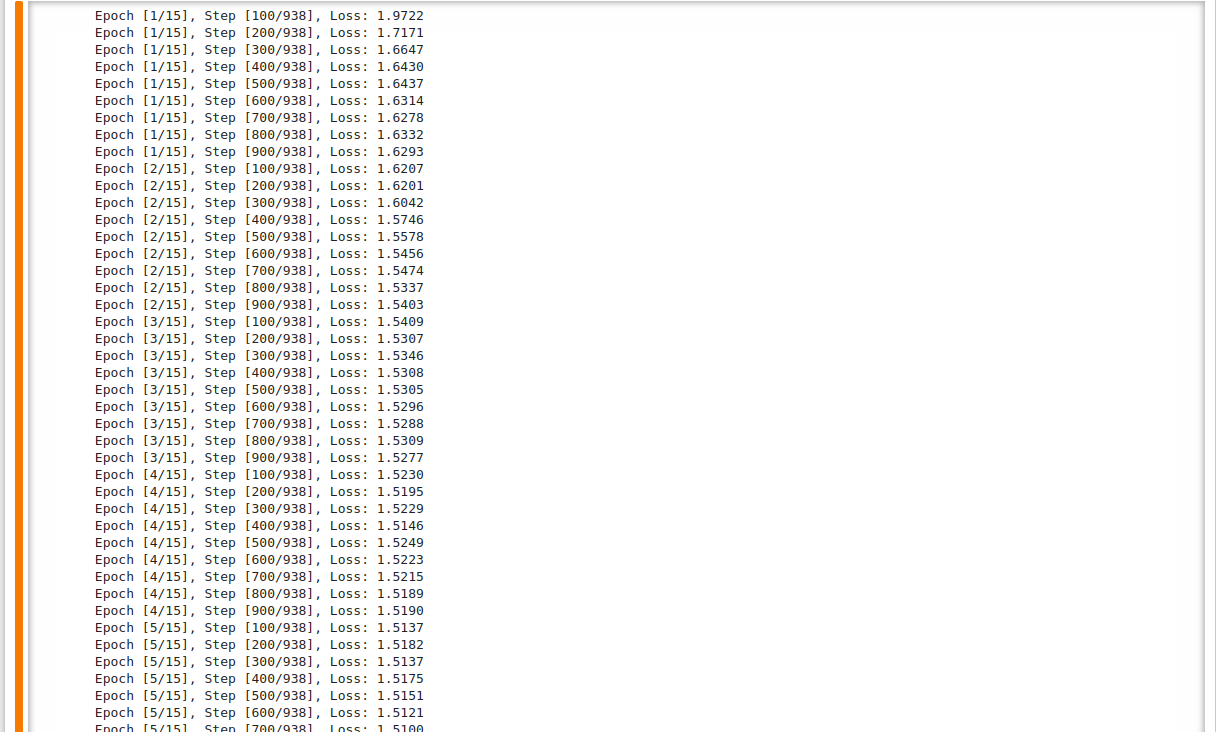
\includegraphics[width=10cm]{Konsolenausgabe_Trainig_neuronales_Netz.png}
\subsection{Testen des Modells}
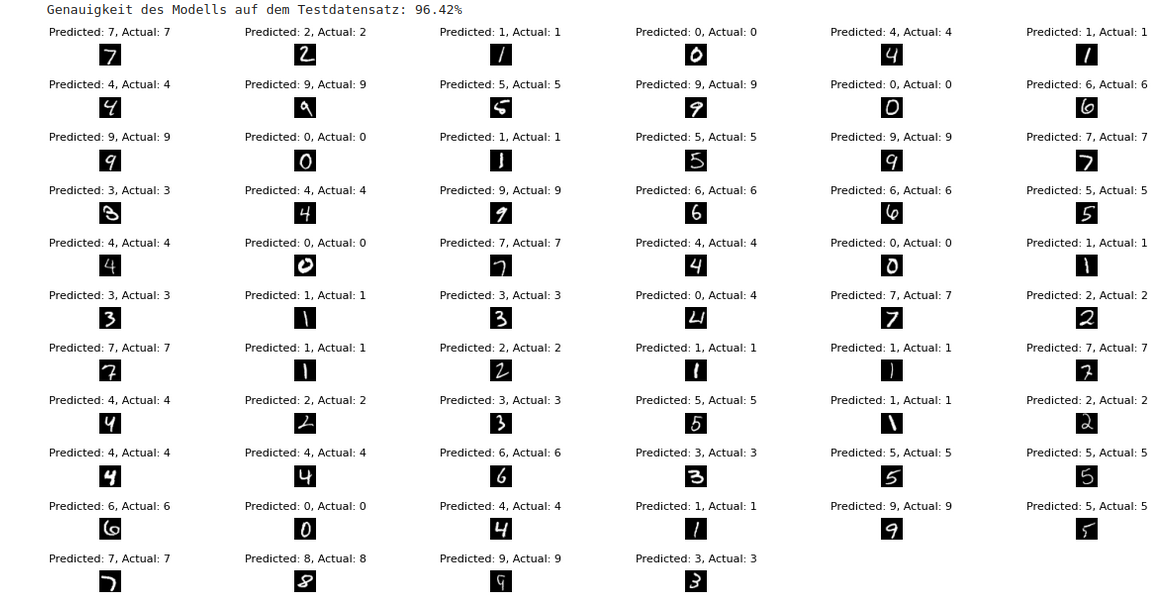
\includegraphics[width=10cm]{Konsolenausgabe_Test_neuronales_Netz.png}
\end{document}
